

\documentclass[12pt]{article}
\usepackage{graphicx}
\usepackage{amsmath}
\usepackage{listings}
\usepackage{color}
\usepackage[section]{placeins} %this stops the figures from showing up in wrong section

\definecolor{dkgreen}{rgb}{0,0.6,0}
\definecolor{dkblue}{rgb}{0,0.0,0.6}
\definecolor{dkred}{rgb}{0.9,0.0,0.1}


\begin{document}

\lstset{language=Fortran,tabsize=4,numbers=left,numberstyle=\tiny,basicstyle=\ttfamily\small\color{dkblue},stringstyle=\ttfamily\color{blue},keywordstyle=\rmfamily\color{dkred}\bfseries\emph,backgroundcolor=\color{white},commentstyle=\color{dkgreen}}




\title{Physics 562 - Computational Physics\\[.5cm]
Final
}
\author{Josh Fernandes\\
Department of Physics \& Astronomy\\
California State University Long Beach}
\date{\today}

  
\maketitle



\begin{abstract}
This paper examines three ways of solving for eigenfunctions. The first problem uses Runge-Kutta to solve for the wave functions of a one-dimensional problem with a coulomb potential. The second problem uses matrices to solve for the same problem. The third problem solves a scattering problem.
\end{abstract}


\section{Problem 1}

The first system is a quantum one-dimensional problem with $\hbar=1$ and $mass=1$. The potential is of the form
\begin{gather}
V(x)=\frac{1}{\sqrt{1+x^2}}.
\end{gather}
The eigenvalues are calculated by assuming the value of the endpoints and using Runge-Kutta to solve for the wave function. Chebyshev is then used to find the energies where either the wave function or the derivative of the wave function vanish at zero. To find orthogonality, use the equation
\begin{gather}
\int_{-\infty}^{+\infty} \psi_n^* \psi_m \,dx = \delta_{nm}.
\label{equationone}
\end{gather}
If $n=m$ integrating over the wave functions will give a value of $1$, otherwise integrating will give a value of $0$.

\subsection{The Fortran95 code}

\begin{lstlisting}[frame=single,caption={program {\tt ho1d.f95}},label=module]


module setup

    use NumType
    implicit none
    integer, parameter  :: n_eq = 3
    real(dp), parameter :: hbar = 1._dp,hbar2 = hbar**2,&
                           mass = 1._dp, omega = 1._dp, &
                           x0 = sqrt(hbar/(mass*omega))
    real(dp) :: energy, xmax, dx, eps, total,val1,val2
    real(dp), allocatable, dimension(:,:) :: wf, w1
    integer :: imax

end module setup

program ho1d

    use setup
    use chebyshev
    implicit none
    real(dp) :: eminx, emaxx, emin, emax, de, e0, de0
    real(dp), external :: psi0
    integer :: nch, iz, i, maxf, izz,m,n,j,k

    eminx = -1._dp
    emaxx = 0._dp

    xmax = 40.0_dp
    dx = 0.01_dp
    eps = 0.000001_dp
    de0 = 0.01_dp
    maxf = 10
    imax = abs(xmax/dx)
    allocate(wf(0:imax,2))
    allocate(w1(0:2*imax,10))
    de = 0.01_dp
    izz = 0
    nch = 5
    emin = eminx
    emax = emin+de

    print *, '================Eigenvalues==============='

    do while (emin < emaxx)

        call chebyex(psi0, nch, cheb, emin, emax)
        call chebyzero(nch,cheb,emin,emax,z0,iz0)

        do iz=1,iz0
            e0=z0(iz)
            call root_polish(psi0,e0,de0,eps,maxf)
            izz = izz + 1
            print *, izz, e0
            call wavef(e0,izz)
        end do
        
        emin = emax
        emax = emin + de

    end do

    print *, '============Orthogonality Test============'

    total = 0
    val1=0
    val2=0
    j=1
    k=1

    do j = 1,10
    do k = 1,10
    do i = 1,2*imax
        m=j
        n=k
        val1=w1(i,m)*w1(i,n)
        val2=w1(i+1,m)*w1(i+1,n)
        !Rombint/trapazoidal method of integration
        total = total + (0.01*(val1+1/2._dp*(val2-val1)))
    end do

    print '(a,1f5.1,a5,i2,a5,i2)','total=', &
    	 total,'i=',j,'j=',k

    total = 0

    end do
    end do



end program ho1d

function psi0(eee) result(psi)

    use setup
    implicit none
    real(dp), intent(in) :: eee
    real(dp) :: x, psi
    real(dp), dimension(n_eq) :: y

    energy = eee
    x = xmax
    y(1) = 0.00001
    y(2) = -0.00001
    y(3) = 0._dp
    do while ( x > 0._dp )
        call rk4step(x,y,-dx)
    end do 
    psi = y(1)*y(2)

end function psi0

subroutine wavef(eee,iz)

    use setup
    implicit none
    real(dp), intent(in) :: eee
    real(dp) :: x, parity
    real(dp), dimension(n_eq) :: y
    integer :: iz, i, imin
    energy = eee
    x = xmax
    y(1) = 0.00001
    y(2) = -0.00001
    y(3) = 0._dp
    do while ( x > 0._dp)
        call rk4step(x,y,-dx)
    end do
   
    x = xmax
    i = imax + 1
    y(1) = 0.00001
    y(2) = -0.00001
    y(3) = 0._dp
    do while ( x > 0._dp)
        i = i-1
        wf(i,1) = x
        wf(i,2) = y(1)
        call rk4step(x,y,-dx)
    end do

    !establish parity so the negative side of 
    !graph can be plotted
    imin=i
    if( abs(y(1)) > abs(y(2)) ) then
        parity = 1
    else 
        parity = -1
    end if 

    ! make a master list of wavefunctions called w1. 
    !Used for integration
    w1(0:imax,iz) = parity*wf(0:imax,2)/sqrt(2*y(3)) 
    w1(imax:2*imax,iz) = wf(0:imax,2)/sqrt(2*y(3)) 

    !normalize the wavefunction
    wf(0:imax,2) = wf(0:imax,2)/sqrt(2*y(3)) 
    

    !make the graphs for positive and negative sides
    do i = imax, imin, -1
        write(unit=20+iz,fmt='(2f15.5)') wf(i,1), &
            wf(i,2)
    end do

    do i = imin, imax
        write(unit=20+iz,fmt='(2f15.5)') -wf(i,1), &
            parity*wf(i,2)
    end do


end subroutine wavef\end{lstlisting}



\section{Problem 2}

The next problem solves the same system as problem 1, but to solve it in the basis of the simple harmonic oscillator.

\subsection{The Fortran95 code}

\begin{lstlisting}[frame=single,caption={ {\tt int.f95}},label=module]

\end{lstlisting}

\section{Problem 3}
The thirds system solves for a quantum scattering system. The wave function vanishes at zero and as $r\rightarrow \infty$ the wave function becomes
\begin{gather}
\psi(r) \sim sin(kr - l\frac{\pi}{2} + \delta_l),
\end{gather}
where
\begin{gather}
k=\sqrt{\frac{2mE}{\hbar^2}}.
\end{gather}
The $l=0$ phase shift are calculated for $E=1,5,10, \& \, 20$. The bound state energies for $l=0$ are also computed. This problem required two different codes. One that is run with {\tt ho1d} to calculate the phase shift and one that is run with {\tt ho2d} to calculate the bound state energies.

\subsection{The Fortran95 code}

\begin{lstlisting}[frame=single,caption={ {\tt ho1d10.f95}},label=module]


module setup

    use NumType
    implicit none
    integer, parameter :: n_eq = 3
    real(dp), parameter :: hbar2=1._dp, &
            mass=1.0_dp, xm=mass*mass/(mass+mass)
    integer :: l

    real(dp) :: energy, xmax, dx, eps, xmid
    real(dp), allocatable, dimension(:,:) :: wf
    integer :: imax

end module setup

program ho1d

    use setup
    use chebyshev
    implicit none
    real(dp) :: dmin,dmax,de,delta0,psi, energy_array(4)
    real(dp), external :: psi0
    integer :: nch, iz, i, maxf

    l=0
    energy_array(1)=1._dp
    energy_array(2)=5._dp
    energy_array(3)=10._dp
    energy_array(4)=20._dp

    xmax=10._dp
    dx=0.001_dp
    eps=0.0000001_dp
    maxf=20
    dmin=0._dp
    dmax=pi

    imax=nint(xmax/dx)+1
    allocate(wf(0:imax,2))

    nch=6

    do i = 1,4
    energy = energy_array(i)
    print *,'for Energy=', nint(energy)
    call chebyex(psi0,nch,cheb,dmin,dmax)
    call chebyzero(nch,cheb,dmin,dmax,z0,iz0)

    de=0.01_dp

    do iz=1,iz0
        delta0=z0(iz)
        call root_polish(psi0,delta0,de,eps,maxf)
        psi=psi0(delta0)
        print *, ' Delta=', delta0
        call wavefunction(delta0,i)
    end do

    end do

end program ho1d

function psi0(delta) result(psi)

    use setup
    implicit none
    real(dp), intent(in) :: delta
    real(dp) :: x, psi, k
    real(dp), dimension(n_eq) :: y

    k = sqrt(2*xm/hbar2*energy)

    x=xmax
    y(1) = sin(k*x - l*pi/2 +delta)
    y(2) = k*cos(k*x -l*pi/2 +delta)
    do while ( x>xmid)
        call rk4step(x,y,-dx)
    end do
    psi=y(2)

end function psi0

subroutine wavefunction(delta,index)

    use setup
    implicit none
    real(dp), intent(in) :: delta
    integer, intent(in) :: index
    real(dp) :: x, k, y12,y11
    real(dp), dimension(n_eq) :: y
    integer :: n, i
    
    k=sqrt(2*xm/hbar2*energy)

    x=xmax
    y(1)=sin(k*x-l*pi/2+delta)
    y(2)=k*cos(k*x-l*pi/2+delta)
    do while (x>xmid)
        n=nint(x/dx)
        wf(n,1)=x
        wf(n,2)=y(1)
        call rk4step(x,y,-dx)
    end do
    y12=y(1)

    wf(0,1)=0._dp
    wf(0,2)=0._dp
    x=dx
    y(1)=x**(l+1)
    y(2)=(l+1)*x**l
    do while (x<=xmid)
        n=nint(x/dx)
        wf(n,1)=x
        wf(n,2)=y(1)
        call rk4step(x,y,dx)
    end do
    y11=y(1)

    wf(0:n,2)=y12/y11*wf(0:n,2)
    n=nint(xmax/dx)
    do i = 0,n
        write(10+index,*) wf(i,1),wf(i,2)
    end do

end subroutine wavefunction


\end{lstlisting}


\begin{lstlisting}[frame=single,caption={ {\tt ho1d10\_energy.f95}},label=module]


module setup

    use NumType
    implicit none
    integer, parameter :: n_eq = 3
    real(dp), parameter :: hbar2=1._dp, &
            mass=1.0_dp, xm=mass*mass/(mass+mass)
    integer :: l

    real(dp) :: energy, xmax, dx, eps, xmid
    real(dp), allocatable, dimension(:,:) :: wf
    integer :: imax

end module setup

program bound

    use setup
    use chebyshev
    implicit none
    real(dp) :: eminx,emin,emaxx,emax,deltae, &
        de,e0,psi
    real(dp), external :: psi0
    integer :: nch, izz, i, maxf, n, nstep

    l=0
    
    xmax=5.0_dp
    dx=0.001_dp
    eps=0.0001_dp
    maxf=20
    eminx=-100._dp
    emaxx=0._dp
    de=0.2_dp
    nstep=5
    nch=5

    imax=nint(xmax/dx)+1
    allocate(wf(0:imax,2))

    e0=eminx
    do
        psi=psi0(e0)
        if(psi /= xmax .or. e0 > emaxx) exit
        e0=e0+de
    end do

    eminx=e0
!     print *, eminx
    deltae=(emaxx-eminx)/nstep
!     print *, deltae

    izz = 0

    print *, 'The bound state energy are '
    do n=1,nstep

        emin = eminx+(n-1)*deltae
        emax = eminx+n*deltae
!         print *, emin, emax
        call chebyex(psi0,nch,cheb,emin,emax)
        call chebyzero(nch,cheb,emin,emax,z0,iz0)
!         print *, z0(1:iz0)

        de=0.1_dp
        do i=1,iz0
            e0=z0(i)
            call root_polish(psi0,e0,de,eps,maxf)
            psi=psi0(e0)
            izz=izz+1
            print *, izz,'E=',e0
            call wavef(e0,izz)
        end do

    end do

end program bound

function psi0(eee) result(psi)

    use setup
    implicit none
    real(dp), intent(in) :: eee
    real(dp) :: x, psi, k
    real(dp), dimension(n_eq) :: y

    energy = eee
    k = sqrt(2*xm/hbar2*(-energy))

    x=dx
    y(1)=x**(l+1)
    y(2)=(l+1)*x**l
    y(3)=0._dp
    do while (x <= xmax .and. y(2) > 0._dp)
        call rk4step(x,y,dx)
    end do

    xmid=x
    if ( xmid >= xmax ) then
        psi=xmax
        return
    end if

    x=xmax
    y(1) = exp(-k*x)
    y(2) = -k*y(1)
    y(3) = 0._dp
    do while (x > xmid)
        call rk4step(x,y,-dx)
    end do
    psi=y(2)

!     print *, e,psi

end function psi0

subroutine wavef(eee,iz)

    use setup
    implicit none
    real(dp), intent(in) :: eee
    real(dp) :: x, psi,k,y12,y32,y11,y31,yy
    real(dp), dimension(n_eq) :: y
    integer :: iz, n, i
    
    energy = eee
    k=sqrt(2*xm/hbar2*(-energy))

    x=xmax
    y(1)=exp(-k*x)
    y(2)=-k*y(1)
    y(3) = 0._dp
    do while (x>xmid)
        n=nint(x/dx)
        wf(n,1)=x
        wf(n,2)=y(1)
        call rk4step(x,y,-dx)
    end do
    y12=y(1)
    y32=-y(3)

    wf(0,1)=0._dp
    wf(0,2)=0._dp
    x=dx
    y(1)=x**(l+1)
    y(2)=(l+1)*x**l
    y(3)=0._dp
    do while ( x <= xmid )
        n=nint(x/dx)
        wf(n,1)=x
        wf(n,2)=y(1)
        call rk4step(x,y,dx)
    end do
    y11=y(1)
    y31=y(3)

    wf(0:n,2)=y12/y11*wf(0:n,2)
    y31=(y12/y11)**2* y31
    yy=y31+y32
    n=nint(xmax/dx)
    wf(0:n,2)=wf(0:n,2)/sqrt(yy)
    do i = 0,n
        write(30*(l+1)+iz,*) wf(i,1),-wf(i,2)
    end do

end subroutine wavef

\end{lstlisting}



\section{Results}

\subsection{Problem 1}
The results from problem 1 give the following energies,
\begin {figure}[!htb]
	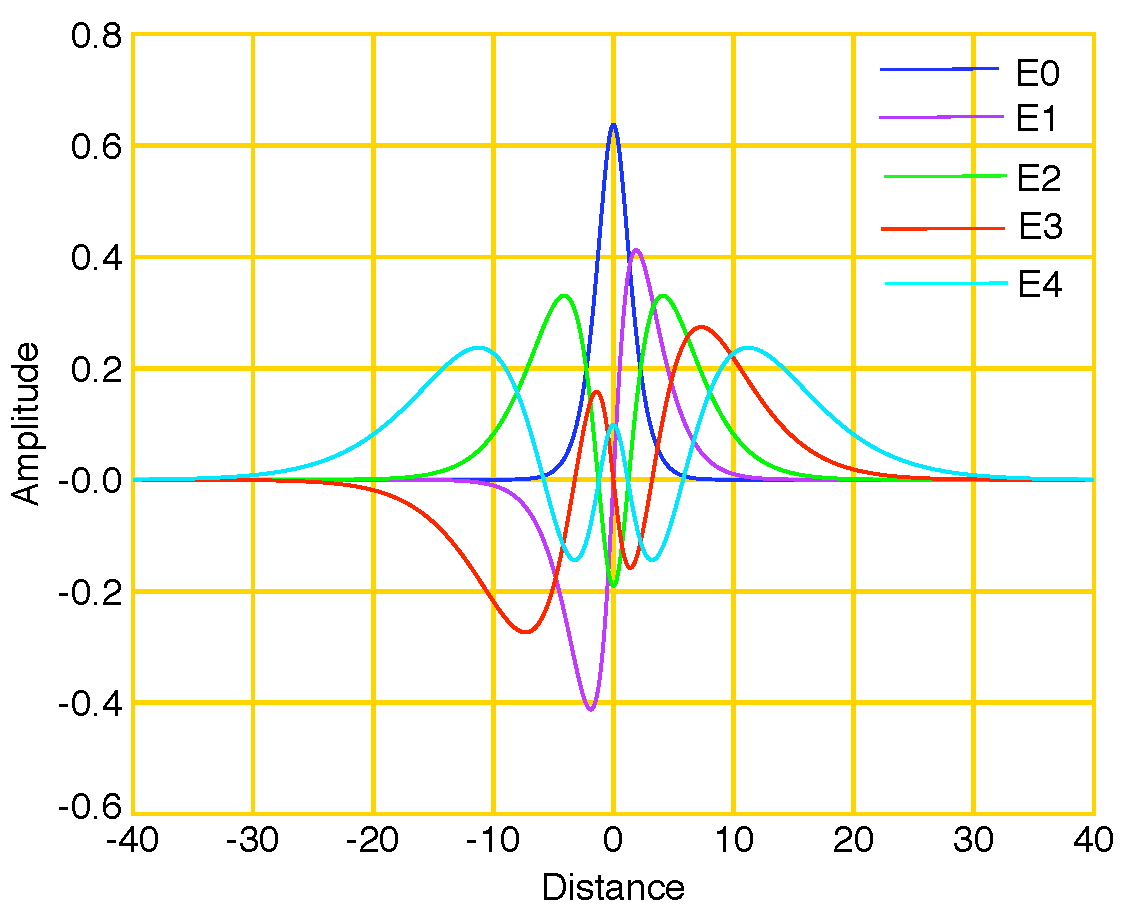
\includegraphics[width=1.\textwidth]{question_1/plot5.pdf}
	%\resizebox{\columnwidth}{!}{\input{question_1/one.png}}
	\caption{The first five wave functions for problem 1 }
	\label{image1one}
\end {figure}  
\begin{align*}
E_0 = -0.669777 \\ 
E_1 = -0.274891 \\
E_2 = -0.151454 \\ 
E_3 = -0.092679 \\
E_4 = -0.063526 \\ 
E_5 = -0.045477 \\
E_6 = -0.034374 \\ 
E_7 = -0.025277 \\
E_8 = -0.016334 \\ 
E_9 = -0.005216
\end{align*}
Notice that as you go up in energy values, the spacing between energy levels gets smaller. The first five wave functions plotted in Fig \ref {image1one}. The eigenstates are also orthogonal as the relationship in Eq. \ref {equationone} holds true. \\

\subsection{Problem 3}
For problem 3, the phase shifts for their respective energies are
\begin{align*}
E = 1,\delta=2.3811  \\ 
E= 5 ,\delta=1.840 \\
E= 10,\delta=1.232 \\ 
E =20,\delta=0.719 
\end{align*}
A completely free particle has a phase shift $\delta_l=0$. The results show that as the energy increases, $\delta_l$ approaches zero. The reason for this is that as a particle has a higher energy, the more easily it can escape from a potential well. The scattering wave functions are plotted in Fig. \ref {image3one}. The bound states for energies for $l=0$ are
\begin{align*}
E_0 = -26.7309  \\ 
E_1 = -13.6180   \\
E_2 = -3.29810
\end{align*}
\begin {figure}[!htb]
	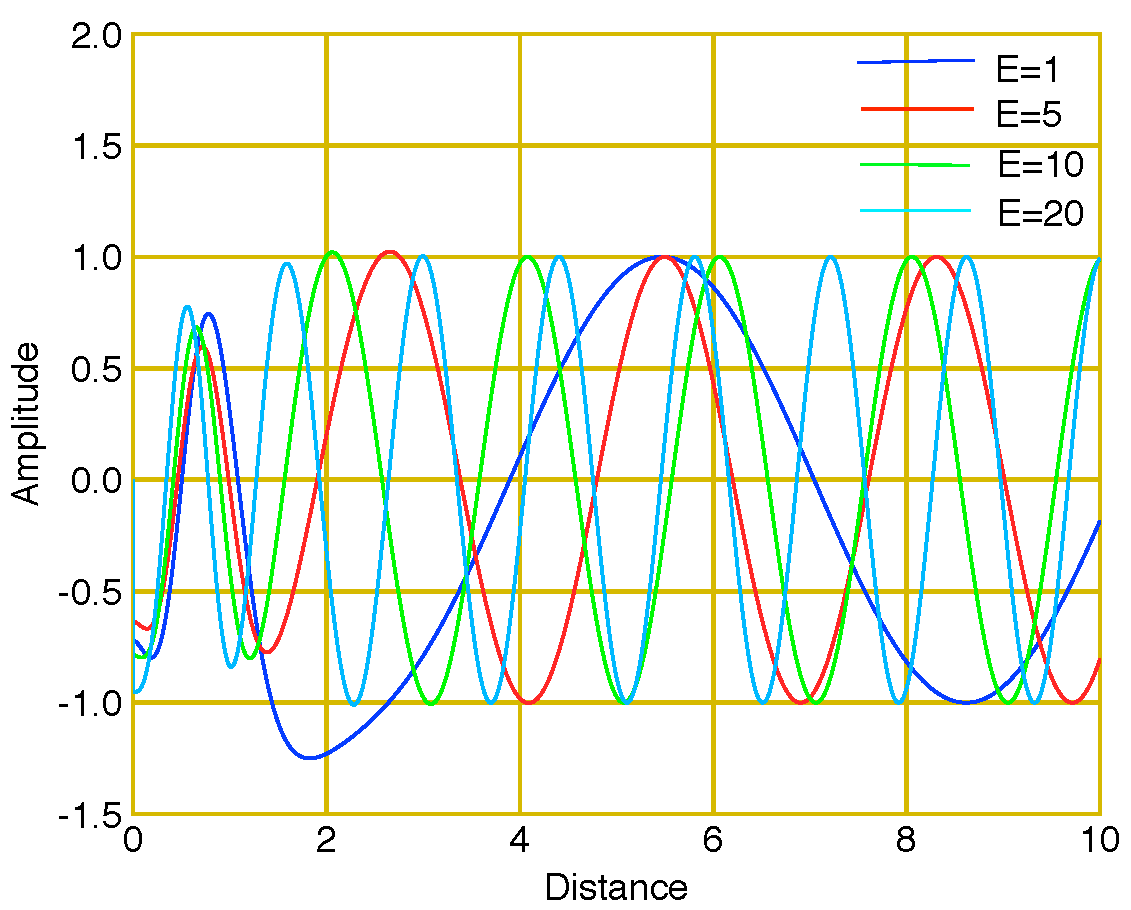
\includegraphics[width=1.\textwidth]{question_3/plot1.pdf}
	%\resizebox{\columnwidth}{!}{\input{question_1/one.png}}
	\caption{The scattering functions for problem 3 }
	\label{image3one}
\end {figure}

\begin {figure}[!htb]
	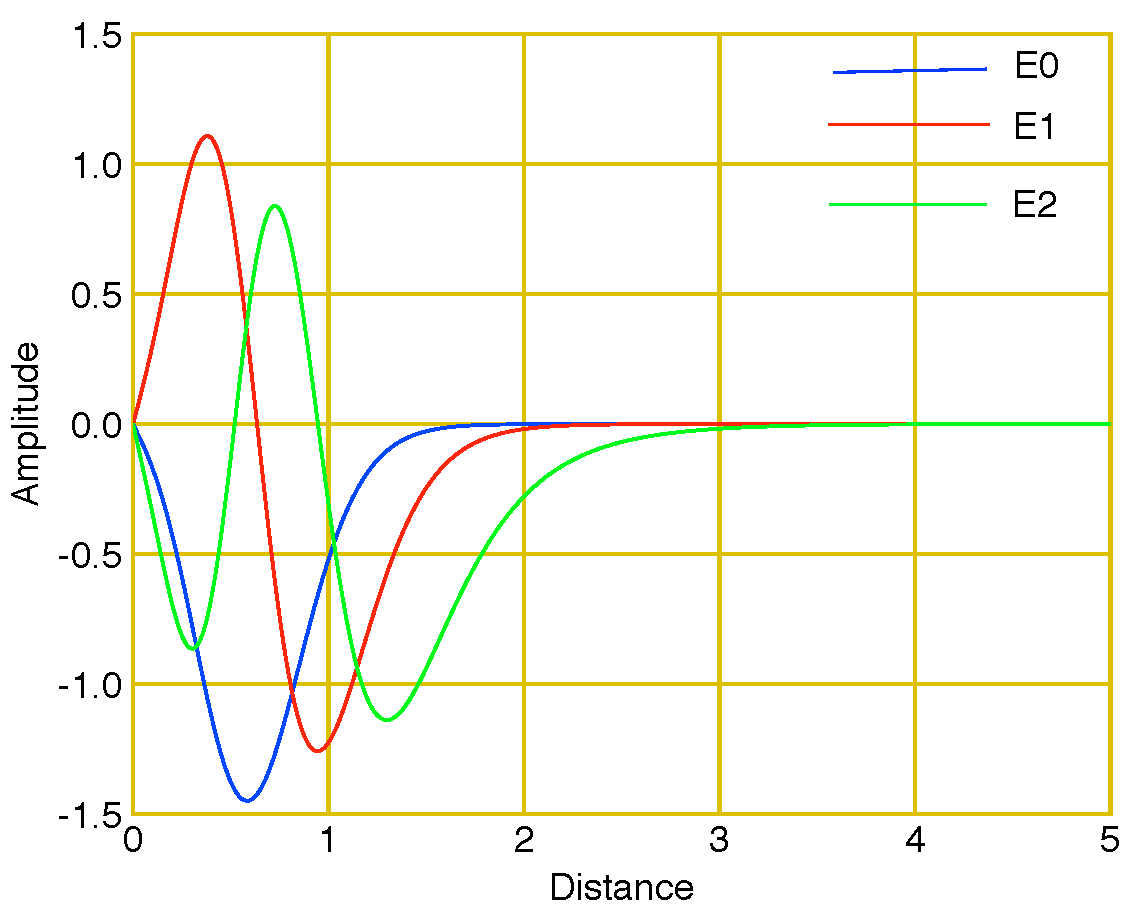
\includegraphics[width=1.\textwidth]{question_3/plot2.pdf}
	%\resizebox{\columnwidth}{!}{\input{question_1/one.png}}
	\caption{The bound functions for problem 3 }
	\label{image3twp}
\end {figure}



\begin{thebibliography}{}


\bibitem{metcalf} M.\ Metcalf, J.\ Reid and M.\ Cohen, {\it Fortran 95/2003 explained}. Oxford University Press, 2004.
 

\end{thebibliography}




\end{document}
